\documentclass{beamer}

\usepackage{graphicx,wrapfig,lipsum}
%\graphicspath{ {images_latex/} }

%\setbeamertemplate{background canvas}{
\includegraphics[width=\paperwidth-100, height=\paperheight]{images_latex/foto.jpg}}

\useoutertheme{infolines}
\usetheme{Hannover}


\title{MyRoute}


\subtitle { \vspace{1cm} \color{black}Juan Germ\'an G\'omez G\'omez \\ \'Alvaro L\'opez Jim\'enez \\ Antonio Jos\'e Camarero Ortega \\ Rub\'en Mar\'in Asunci\'on \\ Rub\'en M\'ogica Garrido \\ Alejandro Ru\'iz Becerra \\ Valent\'in Pedrosa Campoy}

\date{18/01/2019}

\subject{Prácticas DGP}
% This is only inserted into the PDF information catalog. Can be left
% out.

% Delete this, if you do not want the table of contents to pop up at
% the beginning of each subsection:
\AtBeginSubsection[]
{
  \begin{frame}<beamer>{}
    \tableofcontents[currentsection,currentsubsection]
  \end{frame}
}

\begin{document}

\begin{frame}
  \titlepage 
\end{frame}

\begin{frame}{\'Indice}
  \tiny 
  \tableofcontents
  % You might wish to add the option [pausesections]
\end{frame}

% Section and subsections will appear in the presentation overview
% and table of contents.
\section{Gesti\'on del Equipo}

\subsection{Organizaci\'on del Equipo}

\begin{frame}{Titulo diapositiva}{Optional Subtitle}
  \begin{itemize}
  \item {
    My first point.
  }
  \item {
    My second point.
  }
  \end{itemize}
\end{frame}

\subsection{Comunicaci\'on}

\begin{frame}{Comunicaci\'on Externa}
	\begin{figure}[H]
	\centering
	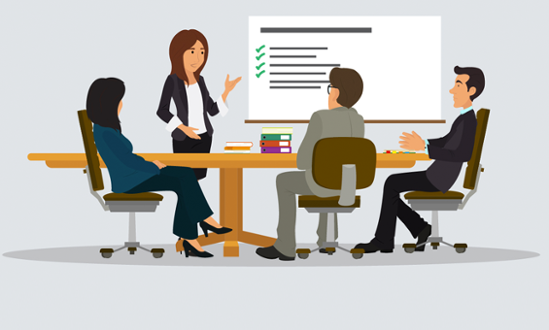
\includegraphics[width=0.35\paperwidth, height=0.4\paperheight]{images_latex/reuniones} 
	\hspace{0.7cm}
	
\includegraphics[width=0.35\paperwidth, height=0.4\paperheight]{images_latex/entrega}
	\end{figure}

\end{frame}

\begin{frame}{Comunicaci\'on Interna}
	\begin{figure}[H]
	\centering
	
\includegraphics[width=0.35\paperwidth, height=0.4\paperheight]{images_latex/reuniones2}
	\hspace{0.7cm}
	
\includegraphics[width=0.35\paperwidth, height=0.4\paperheight]{images_latex/telegram}
	
\includegraphics[width=0.35\paperwidth, height=0.4\paperheight]{images_latex/drive}
	\hspace{0.7cm}
	
\includegraphics[width=0.35\paperwidth, height=0.4\paperheight]{images_latex/github}
	\end{figure}

\end{frame}

\subsection{Seguimiento}

\section{Gesti\'on del Proyecto}

\subsection{Tareas realizadas en cada iteraci\'on}

\subsection{Gesti\'on de la calidad y Accesibilidad}

\section{Arquitectura y tecnolog\'ia}

\subsection{Arquitectura del sistema}

	\begin{frame}{Arquitectura del sistema}
		\begin{itemize}
			\item {
				Back-end : API REST.
				
			}
			\item {
				Front-end : SPA (Single Page Application).
			}
			\item {
				Base de datos : Relacional.
				%\begin{wrapfigure}{r}{0cm}
				%
\includegraphics{images_latex/postgresql}
				%\end{wrapfigure} 
				%
\includegraphics[scale=0.1]{images_latex/postgresql}
				
			}
		\end{itemize}
		
		
		\begin{figure}[h]
			%\hspace{0.3cm}
    		\centering
    		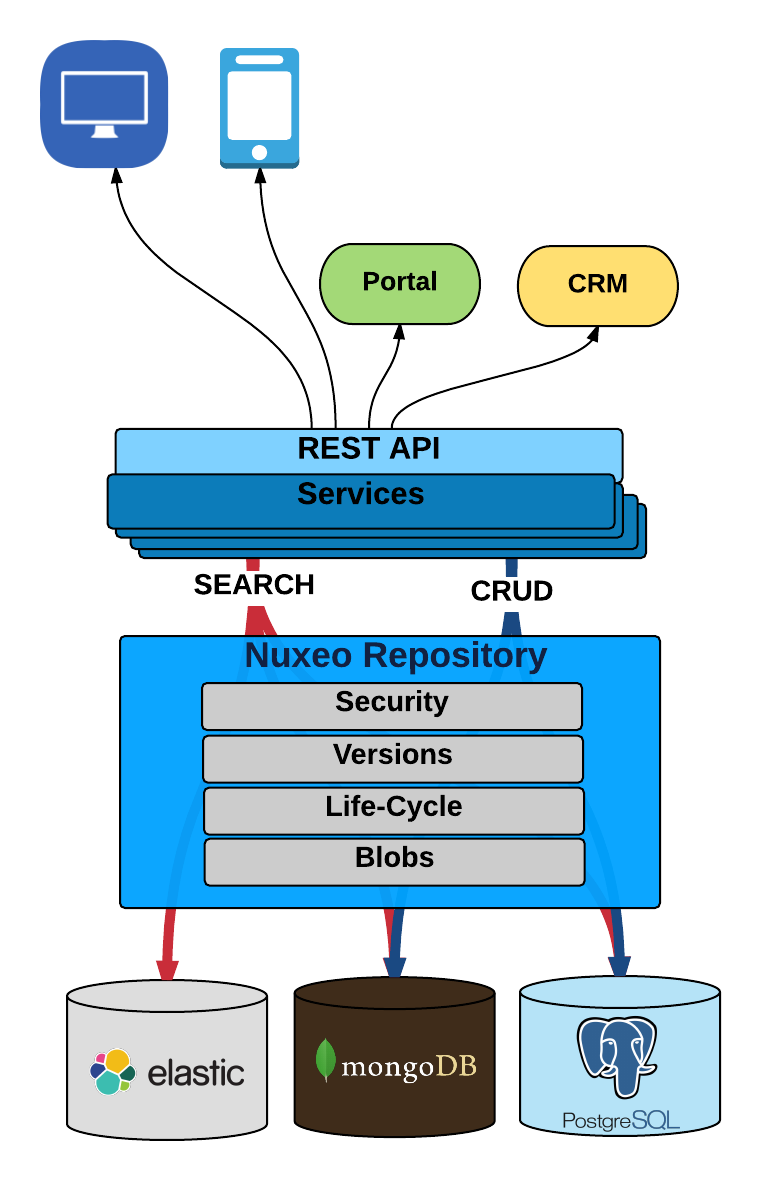
\includegraphics[width=0.7\textwidth, height=0.67\textheight]{images_latex/api}

		\end{figure}
		%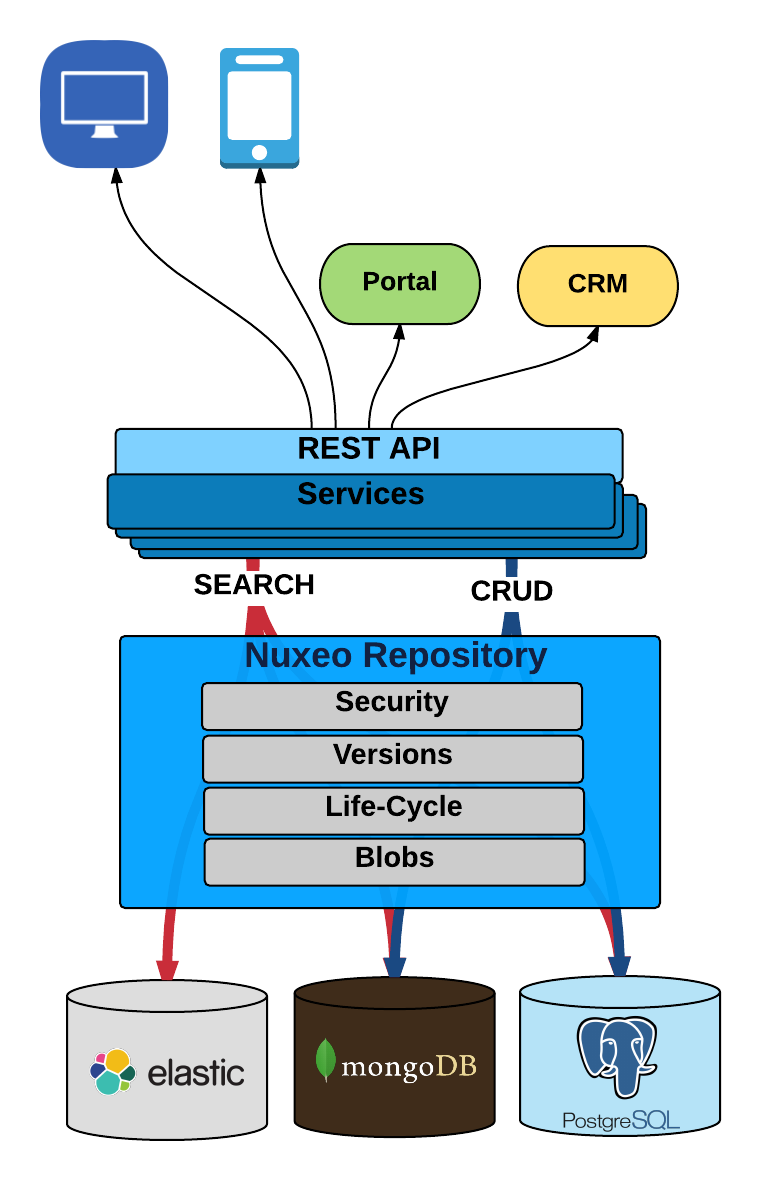
\includegraphics[scale=0.1]{images_latex/api}
	
	\end{frame}

\subsection{Herramientas y tecnolog\'ia}

\section{Pliego T\'ecnico}

\subsection{Cumplimiento del Pliego}

\subsection{Valor A\~nadido}

\section{Retrospectiva}

\subsection{An\'alisis DAFO}

\begin{frame}{An\'alisis DAFO}
	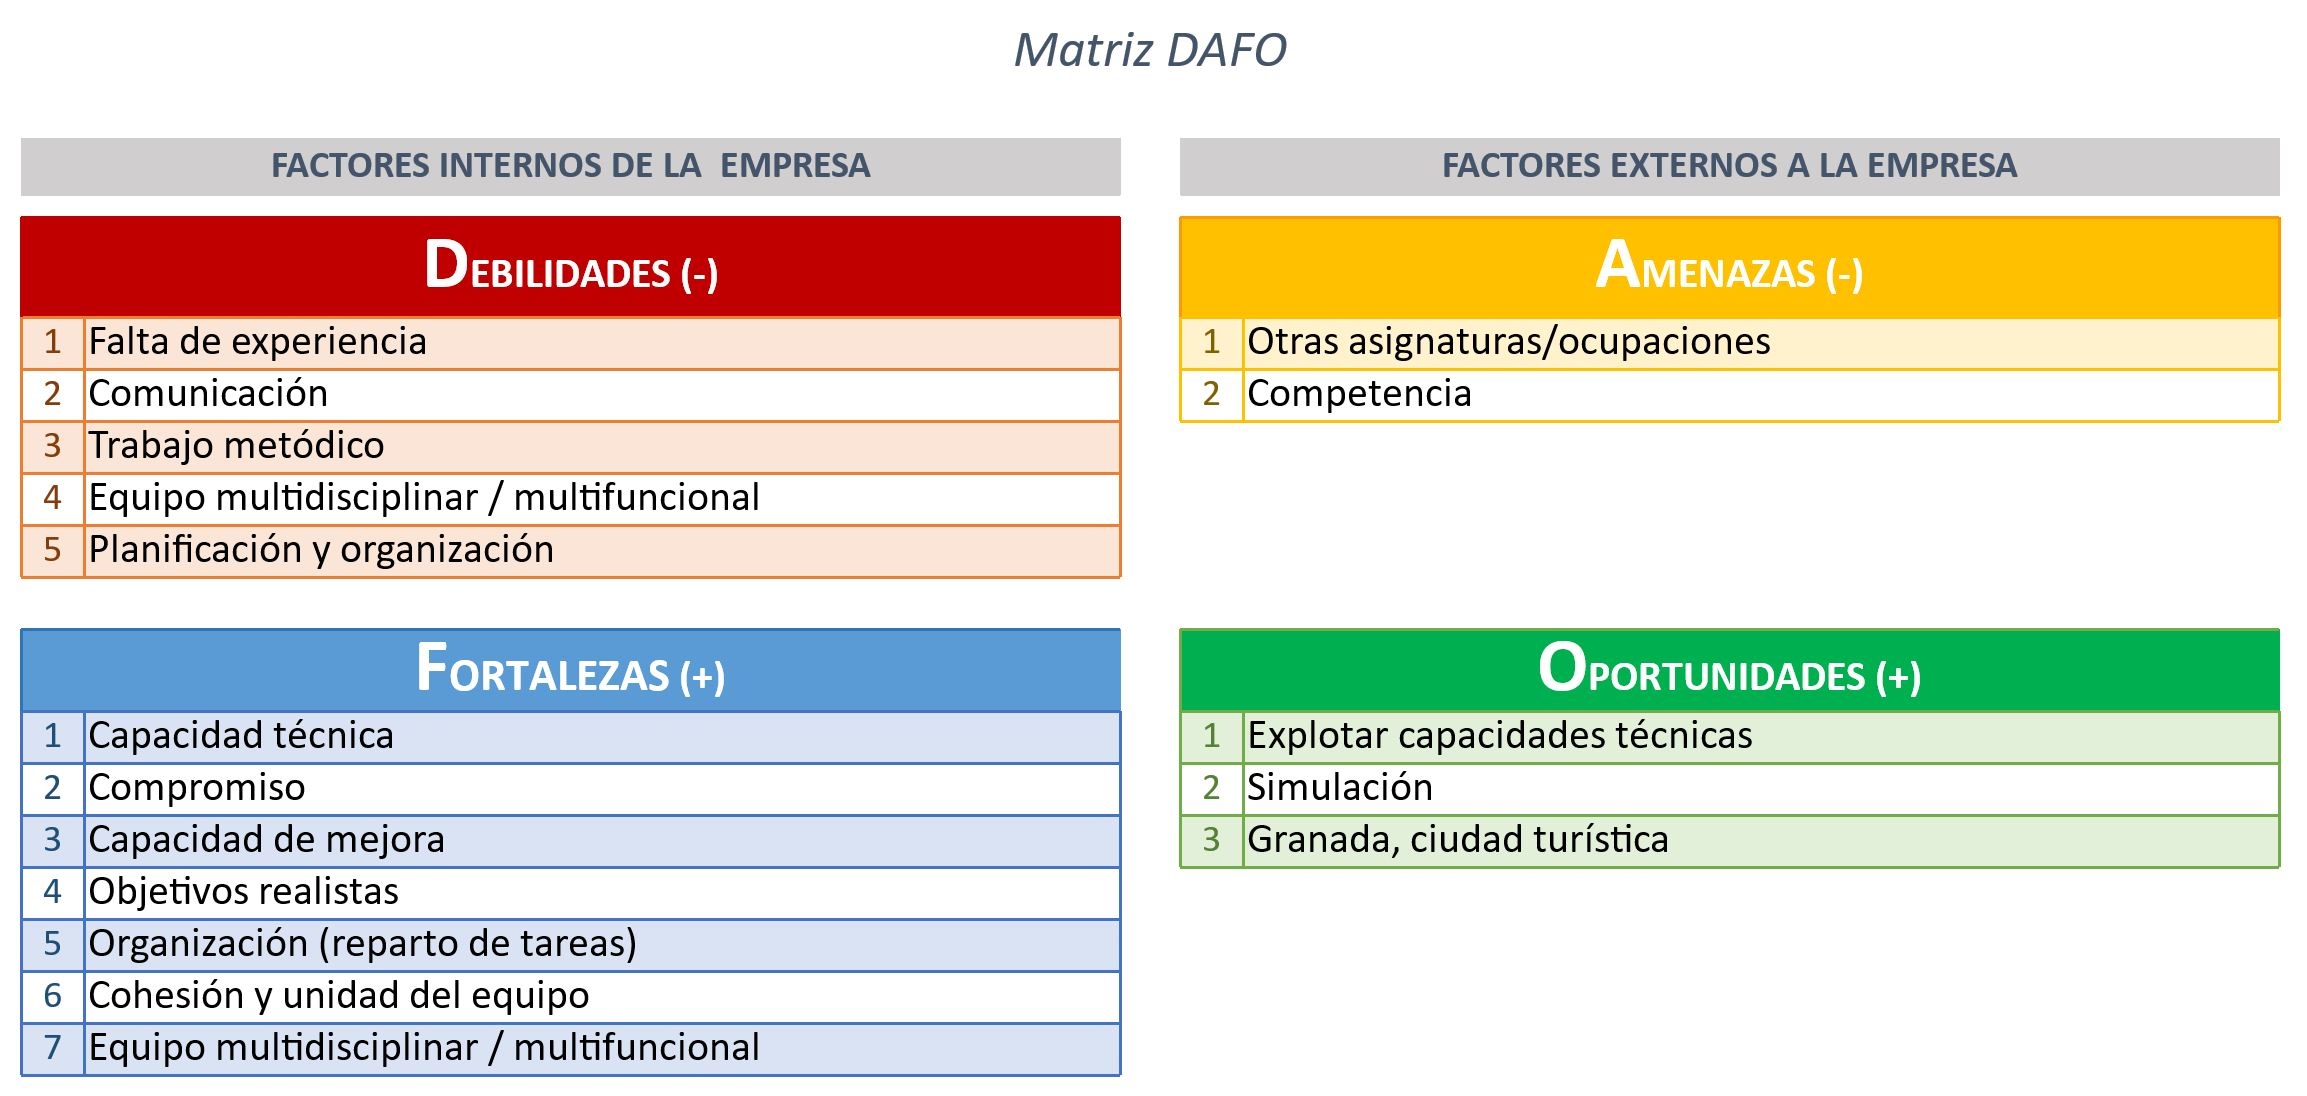
\includegraphics[width=0.8\paperwidth, height=0.8\paperheight]{images_latex/DAFO}
	  
\end{frame}

\subsection{Lecciones aprendidas}

\subsection{Autocr\'itica y cr\'itica a la asignatura}

\begin{frame}{Autocr\'itica}
  \begin{itemize}
  \item { Buen trabajo y buenos resultados. }
  \item { Aspectos a mejorar de cara a futuros proyectos como equipo:
    \begin{itemize}
    \item {Mejorar la comunicaci\'on}
    \item {Ser m\'as met\'odicos}
    \item {Mejorar las habilidades t\'ecnicas de algunos miembros}
    \item {Mejorar la organizaci\'on para evitar bloqueos}
    \end{itemize}
  }
  \end{itemize}
\end{frame}

\begin{frame}{Cr\'itica a la asignatura}
  \begin{itemize}
  \item { ?`C\'omo se gestiona un equipo?}
  \item { ?`C\'omo se gestiona un proyecto?}
  \item {?`C\'omo es trabajar en equipo?}
  \end{itemize}
  
    \begin{itemize}
    \item {No existe jerarqu\'ia}
    \item {Libertad del proyecto y falta de experiencia conlleva confusi\'on}
    \end{itemize}
    
\end{frame}

\subsection{Valoraci\'on Final}

\begin{frame}{Valoraci\'on Final}

\end{frame}

\begin{frame}{Gracias}
	\centering
	
\includegraphics[width=0.6\paperwidth, height = 0.2\paperheight]{images_latex/logo}
\end{frame}


% You can reveal the parts of a slide one at a time
% with the \pause command:
%\begin{frame}{Second Slide Title}
%  \begin{itemize}
%  \item {
%    First item.
%    \pause % The slide will pause after showing the first item
%  }
%  \item {
%    Second item.
%  }
  % You can also specify when the content should appear
  % by using <n->:
%  \item<3-> {
%    Third item.
%  }
%  \item<4-> {
%    Fourth item.
%  }
  % or you can use the \uncover command to reveal general
  % content (not just \items):
%  \item<5-> {
%    Fifth item. \uncover<6->{Extra text in the fifth %item.}
%  }
%  \end{itemize}
%\end{frame}




\end{document}
